\section{Materials and methods}

\subsection{Benchmark conditions and comparison design}
The study examines whether matching one melt-pool length also constrains fusion shape and the rear thermal interval in a conduction model. One source factor is fitted to condition B length. Width and depth are excluded from the fit, and conditions A and C retain the fitted factor. A four-corner comparison at B then changes the high-temperature conductivity and sensible-storage continuations independently. The rear solidus and liquidus positions resolve whether these changes displace the thermal tail or widen the phase interval; their separation and scan speed define a material passage time.

The experimental comparison uses constant-speed laser scanning on bare IN625 plate under three public AMMT conditions (Table~\ref{tab:conditions}). These are single tracks without a powder layer. The three conditions cover increasing speed; A also has a different power, whereas B and C isolate a speed change at fixed nominal power. The reported beam diameter is $D_{4\sigma}=170$~\um. The circular Gaussian reconstruction below uses a radius parameter $w=85$~\um; it does not reproduce the measured two-dimensional beam map.

\begin{table}[htbp]
\centering
\caption{Operating conditions and fixed-source energy scales. The effective factor $\eta\approx0.28905$ is fitted to B length only. $E_\ell=\eta P/v$ and $w/v$ are model input scales.}
\label{tab:conditions}
\begin{tabular}{lrrrr}
\toprule
Condition & $P$ (W) & $v$ (m/s) & $E_\ell$ (J/m) & $w/v$ (\us)\\
\midrule
A & 137.9 & 0.4 & 99.65 & 212.50\\
B & 179.2 & 0.8 & 64.75 & 106.25\\
C & 179.2 & 1.2 & 43.17 & 70.83\\
\bottomrule
\end{tabular}
\end{table}

The length reference is the AMMT condition mean reported by Lane et al.~\cite{lane2020}. Width and depth means are taken from NIST challenge Table~2 for the 100~\us-track microscopy classes~\cite{nist2018}. The latter differ in aggregation and display precision from the subsequently published cross-section means in Lane et al., which combine 100 and 20~\us{} tracks. Length and cross-section references are therefore condition-level quantities from separate observation populations, rather than a joint three-dimensional measurement of one track.

The comparisons are retrospective and nonblind: all public targets were available during development, although only B length enters the calibration objective. Expanded uncertainties $U$ with coverage factor $k=2$ are taken separately from Lane's uncertainty budgets. For width and depth these are descriptive measurement scales from the published combined-class analysis, not uncertainty values jointly estimated with the current decimal NIST means. The ratio $\delta/U$, where $\delta$ is the signed model--reference difference, is used only to report discrepancy scale. It is not a significance test or a combined numerical, input, calibration and measurement uncertainty statistic.

\subsection{Moving-frame enthalpy model and material continuations}
The laboratory-frame conduction balance uses conservative enthalpy~\cite{vanelsen2007}:
\begin{equation}
 \frac{\partial H}{\partial t}=\nabla\cdot[k(T)\nabla T],\qquad
 H(T)=\rho\left[\int_{T_0}^{T}c_p(s)\,\mathrm ds+\mathcal L f(T)\right].
 \label{eq:enthalpy}
\end{equation}
The adopted constants are $\rho=8440$~\si{\kilogram\per\cubic\metre}, $\mathcal L=280000$~\si{\joule\per\kilogram}, $T_0=25$~$^\circ$C, $T_s=1290$~$^\circ$C and $T_l=1350$~$^\circ$C. The adopted linear liquid-fraction closure over the equilibrium melting interval is~\cite{dynamic2024}
\begin{equation}
 f(T)=\begin{cases}
 0,&T<T_s,\\
 (T-T_s)/(T_l-T_s),&T_s\leq T<T_l,\\
 1,&T\geq T_l.
 \end{cases}
\end{equation}
Specific heat and conductivity are linearly interpolated between the input knots in Table~\ref{tab:properties}. The conductivity table contains 15 points and ends at 982~$^\circ$C; the 12-point specific-heat table ends at 1093~$^\circ$C. The supplier labels its typical specific heats as calculated and conductivity as measured~\cite{specialmetals625}; these are general alloy data, not measurements on the benchmark coupon. Density and the melting interval use that bulletin, while the adopted latent heat follows the benchmark modeling setup~\cite{kollmannsberger2019}. The sensible enthalpy integral is evaluated piecewise analytically; adding the phase contribution preserves a monotone temperature--enthalpy relation and permits analytic inversion. The latent contribution to effective specific heat inside the phase interval is 4666.67~\si{\joule\per\kilogram\per\kelvin}.

Both property tables end below the adopted solidus, so the melting-range solution requires a high-temperature continuation (Fig.~\ref{fig:properties}).

\begin{figure}[htbp]
\centering
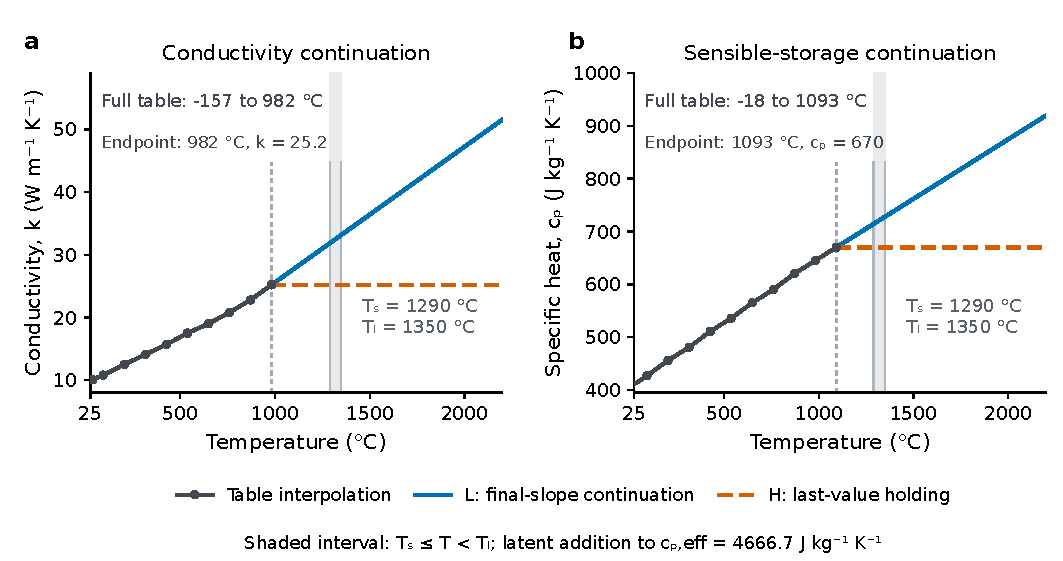
\includegraphics[width=\textwidth]{figures/ammt-property-continuations.pdf}
\caption{Actual IN625 property inputs and the two continuation choices. (a) Conductivity and (b) sensible specific heat use the input knots listed in Table~\ref{tab:properties}, with common piecewise-linear interpolation below the respective endpoints. The final knots are 982~$^\circ$C and 25.2~\si{\watt\per\metre\per\kelvin} for $k$, and 1093~$^\circ$C and 670~\si{\joule\per\kilogram\per\kelvin} for $c_p$. L continues the final tabulated secant; H holds the final value. The displayed window is 25--2200~$^\circ$C; all 15 conductivity and 12 specific-heat source rows, including those below 25~$^\circ$C, are retained in the accompanying data and used in interpolation. Shading marks the adopted 1290--1350~$^\circ$C phase interval. The latent addition to effective specific heat within this interval is 4666.7~\si{\joule\per\kilogram\per\kelvin} and is stated separately from sensible $c_p$. The supplier describes conductivity as measured and specific heat as calculated typical alloy data~\cite{specialmetals625}; the plotted high-temperature continuations are modeling choices.}
\label{fig:properties}
\end{figure}

Two binary factors replace linear continuation (L) by holding the last tabulated value (H), independently for $k$ and $c_p$. H holds $k=25.2$~\si{\watt\per\metre\per\kelvin} above 982~$^\circ$C and $c_p=670$~\si{\joule\per\kilogram\per\kelvin} above 1093~$^\circ$C. The final table secants used for L are $(25.2-22.8)/(982-871)=0.0216216$~W\,m$^{-1}$\,K$^{-2}$ and $(670-645)/(1093-982)=0.225225$~J\,kg$^{-1}$\,K$^{-2}$. The changes apply above each table endpoint, including the solid range between the endpoint and $T_s$. Each conductivity branch changes $k$, its primitive $K$ and the surface inverse together; each storage branch changes $c_p$, $H$ and $T(H)$ together. The first letter labels conductivity. The baseline uses linear continuation for both properties (LL); HL and LH change one property, and HH changes both. The calibration and fixed-source contrasts are defined below.

For a locally quasi-steady translating field, define $\xi=x-vt$ and $\bm u=(-v,0,0)$. Equation~\eqref{eq:enthalpy} becomes
\begin{equation}
 \nabla\cdot(\bm uH-k\nabla T)=0.
 \label{eq:frame}
\end{equation}
The term $\bm uH$ represents stationary material passing through the laser coordinate frame. No liquid momentum equation or melt convection is included. The assumptions also exclude evaporation and free-surface deformation.

With the circular Gaussian $D_{4\sigma}$ convention~\cite{dynamic2024}, the surface input at $z=0$ is
\begin{equation}
 q(\xi,y)=\frac{2\eta P}{\pi w^2}
 \exp\!\left[-\frac{2(\xi^2+y^2)}{w^2}\right].
 \label{eq:source}
\end{equation}
With outward normal $\bm n$, the top condition is $-k\nabla T\cdot\bm n=-q$; the Gaussian supplies inward heat. Its full-plane integral is $\eta P$; the appendix gives the discrete source integration. At positive $\xi$, incoming material has $H=0$; at negative $\xi$, diffusive gradient vanishes and enthalpy leaves advectively. The $y=0$ plane is symmetric. Outer transverse and bottom boundaries are adiabatic. Radiation and ambient convection are omitted from the solved balance.

\subsection{Melt-pool geometry and material passage}
Model length $L$ is the distance between two solidus crossings of the recovered surface symmetry-centerline temperature. Crossings are interpolated, must enclose the source, and must form one interval without domain truncation. Surface and symmetry-plane recovery precede threshold extraction; the appendix gives their numerical definitions.

Fusion-zone width and depth are extracted from the source-connected component of
\begin{equation}
 T_{\max}(y,z)=\max_\xi T(\xi,y,z)\geq T_s.
 \label{eq:fusion}
\end{equation}
Each $\xi$ slice is first reconstructed at the surface and symmetry plane, then bilinearly interpolated onto observation coordinates, and only then maximized over passage. Taking a nodal maximum before interpolation creates a different envelope. Width is twice the positive-$y$ extent and depth is the negative of the lowest $z$. The observation pitch samples interpolated geometry and does not define the heat-field resolution. Figures label the surface length proxy $L_s$ and fusion-envelope extents $W_f$ and $D_f$; these correspond to $L$, $W$ and $D$ in the text.

Lane's imaging length uses a radiance-profile second-derivative minimum for the rear solidification location and a calibrated front threshold~\cite{lane2020}. The present two-solidus-crossing proxy does not replay radiance, emittance, pixel integration, viewing geometry or motion blur. Its fitted $\eta$ is therefore an effective source/model/operator parameter. Width and depth refer instead to a maximum-temperature fusion envelope, compared with metallography.

Let $\xi_s^-$ and $\xi_l^-$ denote the rear centerline solidus and liquidus crossings. Define the rear spatial phase span, passage time and interval-mean cooling rate as
\begin{equation}
 \ell_m=\xi_l^- -\xi_s^-,\qquad
 \tau_m=\frac{\ell_m}{v},\qquad
 \overline{\dot T}=\frac{T_l-T_s}{\tau_m}.
 \label{eq:passage}
\end{equation}
These quantities describe stationary material passing through the same quasi-steady field; they are derived quantities rather than independent thermal observations. The cooling interval is 1350--1290~$^\circ$C and differs from the below-solidus example interval used by Lane.

\subsection{Calibration, constitutive contrasts and numerical adequacy}
Fitting $L_B(\eta)=359$~\um{} gives $\eta\approx0.28905$, with a signed length residual of +0.158~\um. Conditions A and C retain this value, beam, phase law and property continuations. The appendix gives the scalar calibration algorithm, trial values and local sensitivity.

For the four B corners, power, speed, beam, density, phase thresholds, latent heat, mesh and observation operators remain fixed, and no corner is recalibrated. The first letter denotes conductivity and the second sensible specific heat. Sharing B=LL between the operating-condition and continuation comparisons gives six production solutions.

For any output $Q$, define the baseline-anchored finite effects
\begin{align}
 \delta_k&=Q_{\HL}-Q_{\LL}, &
 \delta_{c_p}&=Q_{\LH}-Q_{\LL},\\
 I_{k,c_p}&=Q_{\HH}-Q_{\HL}-Q_{\LH}+Q_{\LL}, &
 \Delta_{\rm joint}&=Q_{\HH}-Q_{\LL}=\delta_k+\delta_{c_p}+I_{k,c_p}.
 \label{eq:contrast}
\end{align}
The conditional conductivity effect at held $c_p$ is $Q_{\HH}-Q_{\LH}=\delta_k+I_{k,c_p}$; the conditional storage effect at held $k$ is $Q_{\HH}-Q_{\HL}=\delta_{c_p}+I_{k,c_p}$. Reporting both conditions checks whether a direction changes with the other factor. These deterministic contrasts distinguish two continuation choices within the same model. They are not estimates from replicated material experiments and have no sampling-significance interpretation.

An axial-face P\'eclet diagnostic compares coordinate enthalpy transport with diffusion in the phase interval. A discrete rear hot-region budget measures net outward diffusive power. Both use temperature-selected regions that can change between branches, so they complement matched-coordinate thresholds rather than supply a fixed-region causal contrast. Their definitions are given in the appendix.

The conservative finite-volume solution uses near-source cell widths of $4\times3\times1$~\um. The graded-domain geometry and enthalpy discretization are specified in the appendix. Convergence is checked using both the sum of absolute cell residuals and the signed global energy balance, followed by a full frozen-coefficient correction.

A separate constant-property moving-Gaussian problem checks source integration, frame transport and geometric extraction against a semi-infinite analytical reference~\cite{oberkampf2002}. Its reference $L/W/D$ is $407.535/153.293/34.836$~\um; finite-volume differences are +0.139\%, +0.190\% and $-0.499$\%, respectively. This simpler comparison does not establish nonlinear phase-change accuracy.

At the calibrated $\eta$, reducing the near-source axial spacing from 4 to 2~\um\ changes B length, width and depth by +0.361, $-0.009$ and +0.041~\um, and C by +0.199, $-0.029$ and +0.045~\um. A/B domain enlargement changes these quantities by less than $3\times10^{-6}$~\um. These measured sensitivities support comparison with the larger geometric responses, but do not give a full three-dimensional error bound for each continuation branch. Submicrometre interactions are therefore reported descriptively. An earlier transient B comparison at a different calibration stage provides only approximate local steady consistency. Fixed-field blackbody estimates put B-corner top losses at 0.099--0.180\% of absorbed power; feedback from these losses is not solved.

All six solutions satisfy the stated energy-balance and nonlinear-correction criteria and give bounded phase fractions and nontruncated extracted geometry. The appendix reports the acceptance thresholds and final residuals.
